\documentclass{article}

\usepackage{amsmath}
\usepackage{amssymb}
\usepackage{amsfonts}
\usepackage[margin=1in]{geometry}
\usepackage{titling}
\usepackage{shellesc}
\usepackage{minted}
\usepackage{graphicx}
\usepackage{siunitx}
\usepackage[bookmarks]{hyperref}
\usepackage{xcolor}
\hypersetup{
    colorlinks,
    linkcolor={red},
    citecolor={blue!50!black},
    urlcolor={blue!80!black}
}

\setlength{\droptitle}{-7em}

\title{Supporting Calculations}
\author{Group 701: Tyler Tian, Julia Ye, Ivy Tan}

\begin{document}

\maketitle
\sloppy

\section{Source Code}

The code is split into two parts: A Python module that does all the calculations (\ref{sec:calc}), and another module
that provides a command-line interface (CLI) (\ref{sec:cli}).

Bridge designs are given to the program in YAML files. The specification for Design 0 (\ref{sec:design0}) and the final
design (\ref{sec:design}) are listed here.

The code depends on the following packages:
\begin{itemize}
    \setlength\itemsep{0em}
    \item \texttt{numpy}
    \item \texttt{matplotlib}
    \item \texttt{pyyaml}
    \item \texttt{click} (CLI only)
\end{itemize}

\subsection{Calculations Code (\texttt{calculate.py})}
\label{sec:calc}

Sample usage of the functions to do the calculations is included at the end of this code listing. All functions are
documented with docstrings, which includes example calls.

\inputminted[linenos, breaklines, fontsize=\small]{python}{../../calculate.py}
\pagebreak

\subsection{Command-Line Interface Code (\texttt{bridgedesigner.py})}
\label{sec:cli}

\inputminted[linenos, breaklines, fontsize=\small]{python}{../../bridgedesigner.py}
\pagebreak

\subsection{Bridge Specification Code}

\subsubsection{Design 0 (\texttt{design0.yaml})}
\label{sec:design0}

\inputminted[linenos, breaklines, fontsize=\small]{yaml}{../../design0.yaml}
\pagebreak

\subsubsection{Final Design (\texttt{bridge.yaml})}
\label{sec:design}

\inputminted[linenos, breaklines, fontsize=\small]{yaml}{../../new.yaml}
\pagebreak

\section{Handwritten Calculations}

Manual calculations are shown below for verification of the code. All calculations are for Design 0.

\subsection{Internal Forces}

Verifies reaction forces, shear force diagrams, and bending moment diagrams as computed by
\mintinline{python}{Bridge.reaction_forces()}, \mintinline{python}{Bridge.make_sfd()}, and
\mintinline{python}{Bridge.make_bmd()}. These numbers can be obtained by running
\texttt{python3 bridgedesigner.py design0.yaml load point 200}.

\begin{figure}[h]
    \centering
    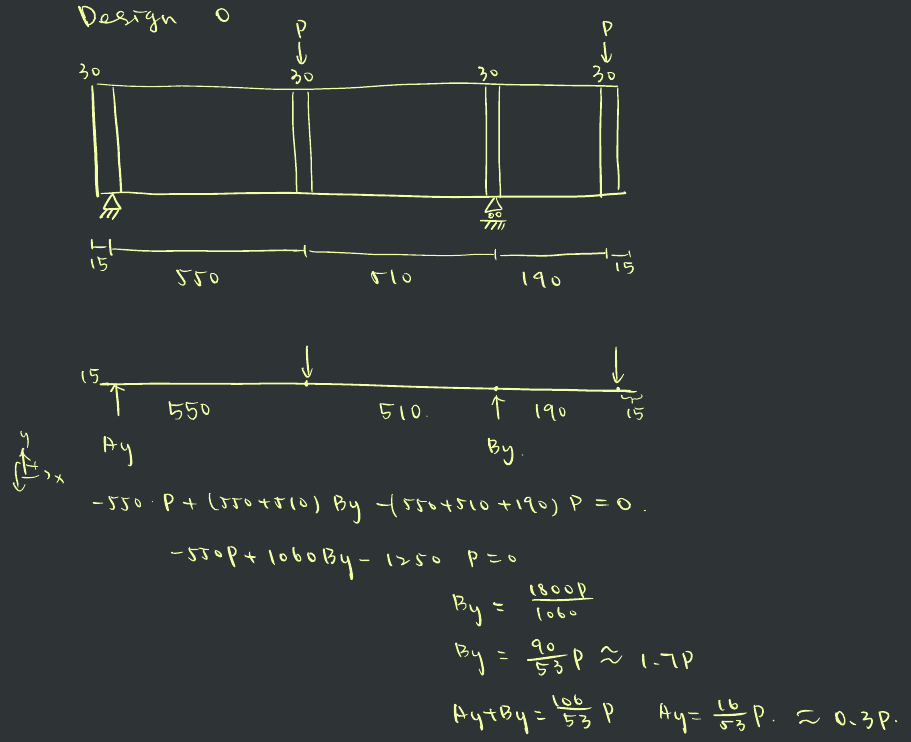
\includegraphics[width=0.49\textwidth]{forces.png}
    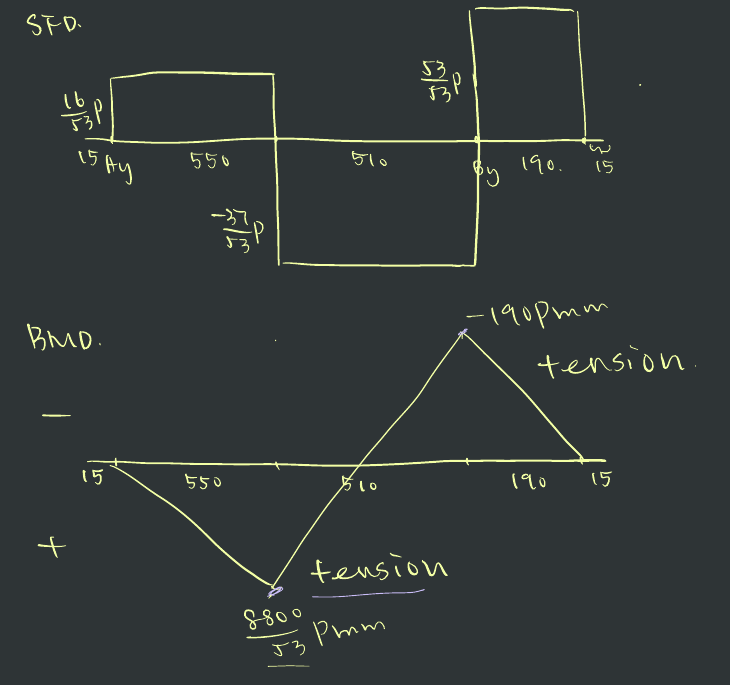
\includegraphics[width=0.49\textwidth]{sfd_bmd.png}
    \caption{Reaction forces, SFD and BMD (point loading).}
\end{figure}

\subsection{Cross-Sectional Properties}

Verifies cross-sectional properties computed by the \mintinline{python}{CrossSection} class.
These numbers can be obtained by running \texttt{python3 bridgedesigner.py design0.yaml geometry}.

\begin{figure}[h]
    \centering
    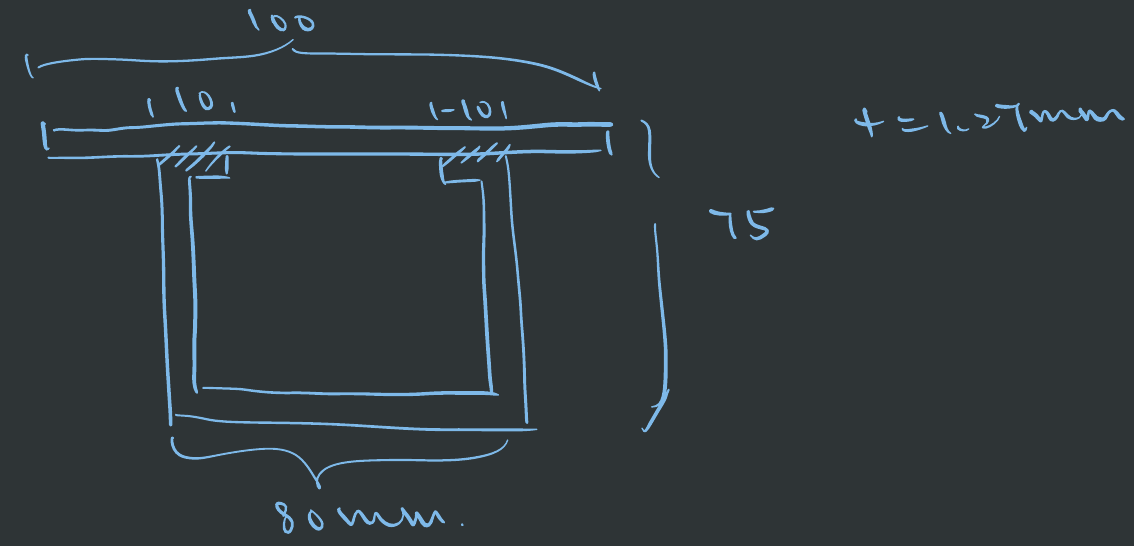
\includegraphics[width=0.5\textwidth]{cs.png}
    \caption{Cross-sectional geometry.}
\end{figure}

\begin{align*}
    A &= 100t + 2 \cdot 10t + 2 \cdot (75 - t)t + (80 - 2t)t = 438\si{mm^2} \\
    \bar{y} &= \frac{100t\left(75 - \frac{t}{2}\right) + 2 \cdot 10t(75 - t - \frac{t}{2}) + 2 \cdot (75 - t)t\frac{75 - t}{2} + (80 - 2t)t\frac{t}{2}}{A} = 41.7\si{mm}\\
    I &= \frac{100t^3}{12} + 100t\left(75 - \frac{t}{2} - \bar{y}\right)^2 \\
        & + 2\left(\frac{10t^3}{12} + 10t\left(75 - t - \frac{t}{2} - \bar{y}\right)^2 + \frac{t(75 - t)^2}{12} + (75 - t)t\left(\frac{75 - t}{2} - \bar{y}\right)^2\right) \\
        &+ \frac{(80 - 2t)t^3}{12} + (80 - 2t)t\left(\frac{t}{2} - \bar{y}\right)^2 \\
      &= \SI{416e3}{mm^4}
\end{align*}

\begin{figure}[h]
    \centering
    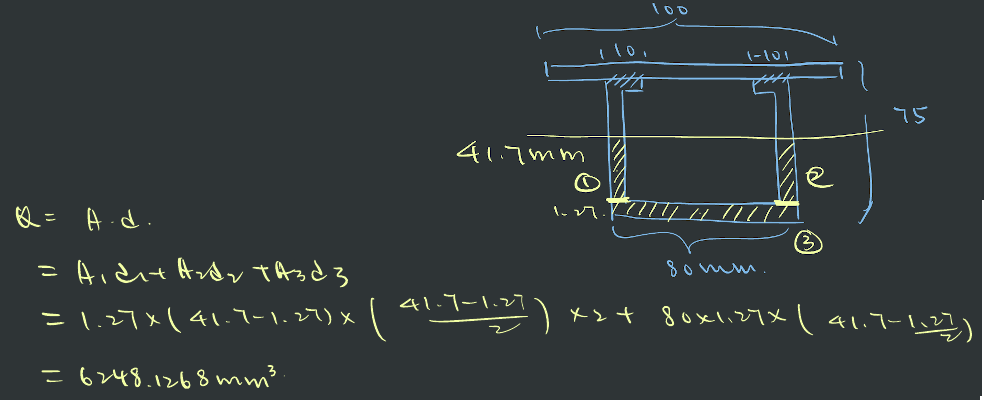
\includegraphics[width=0.7\textwidth]{qcent.png}
    \caption{Computing \(Q\) at the centroidal axis.}
\end{figure}

\subsection{Bridge Capacity}

Verifies various \(M_{fail}\) and \(V_{fail}\) values as computed by the \mintinline{python}{Bridge.calculate_<mode>_mfail()}
and \mintinline{python}{Bridge.calculate_<mode>_vfail()} methods. These numbers can be obtained by running
\texttt{python3 bridgedesigner.py design0.yaml load point 200 --mfail all --vfail all}.

\subsubsection{Shear Failure}

\begin{figure}[H]
    \centering
    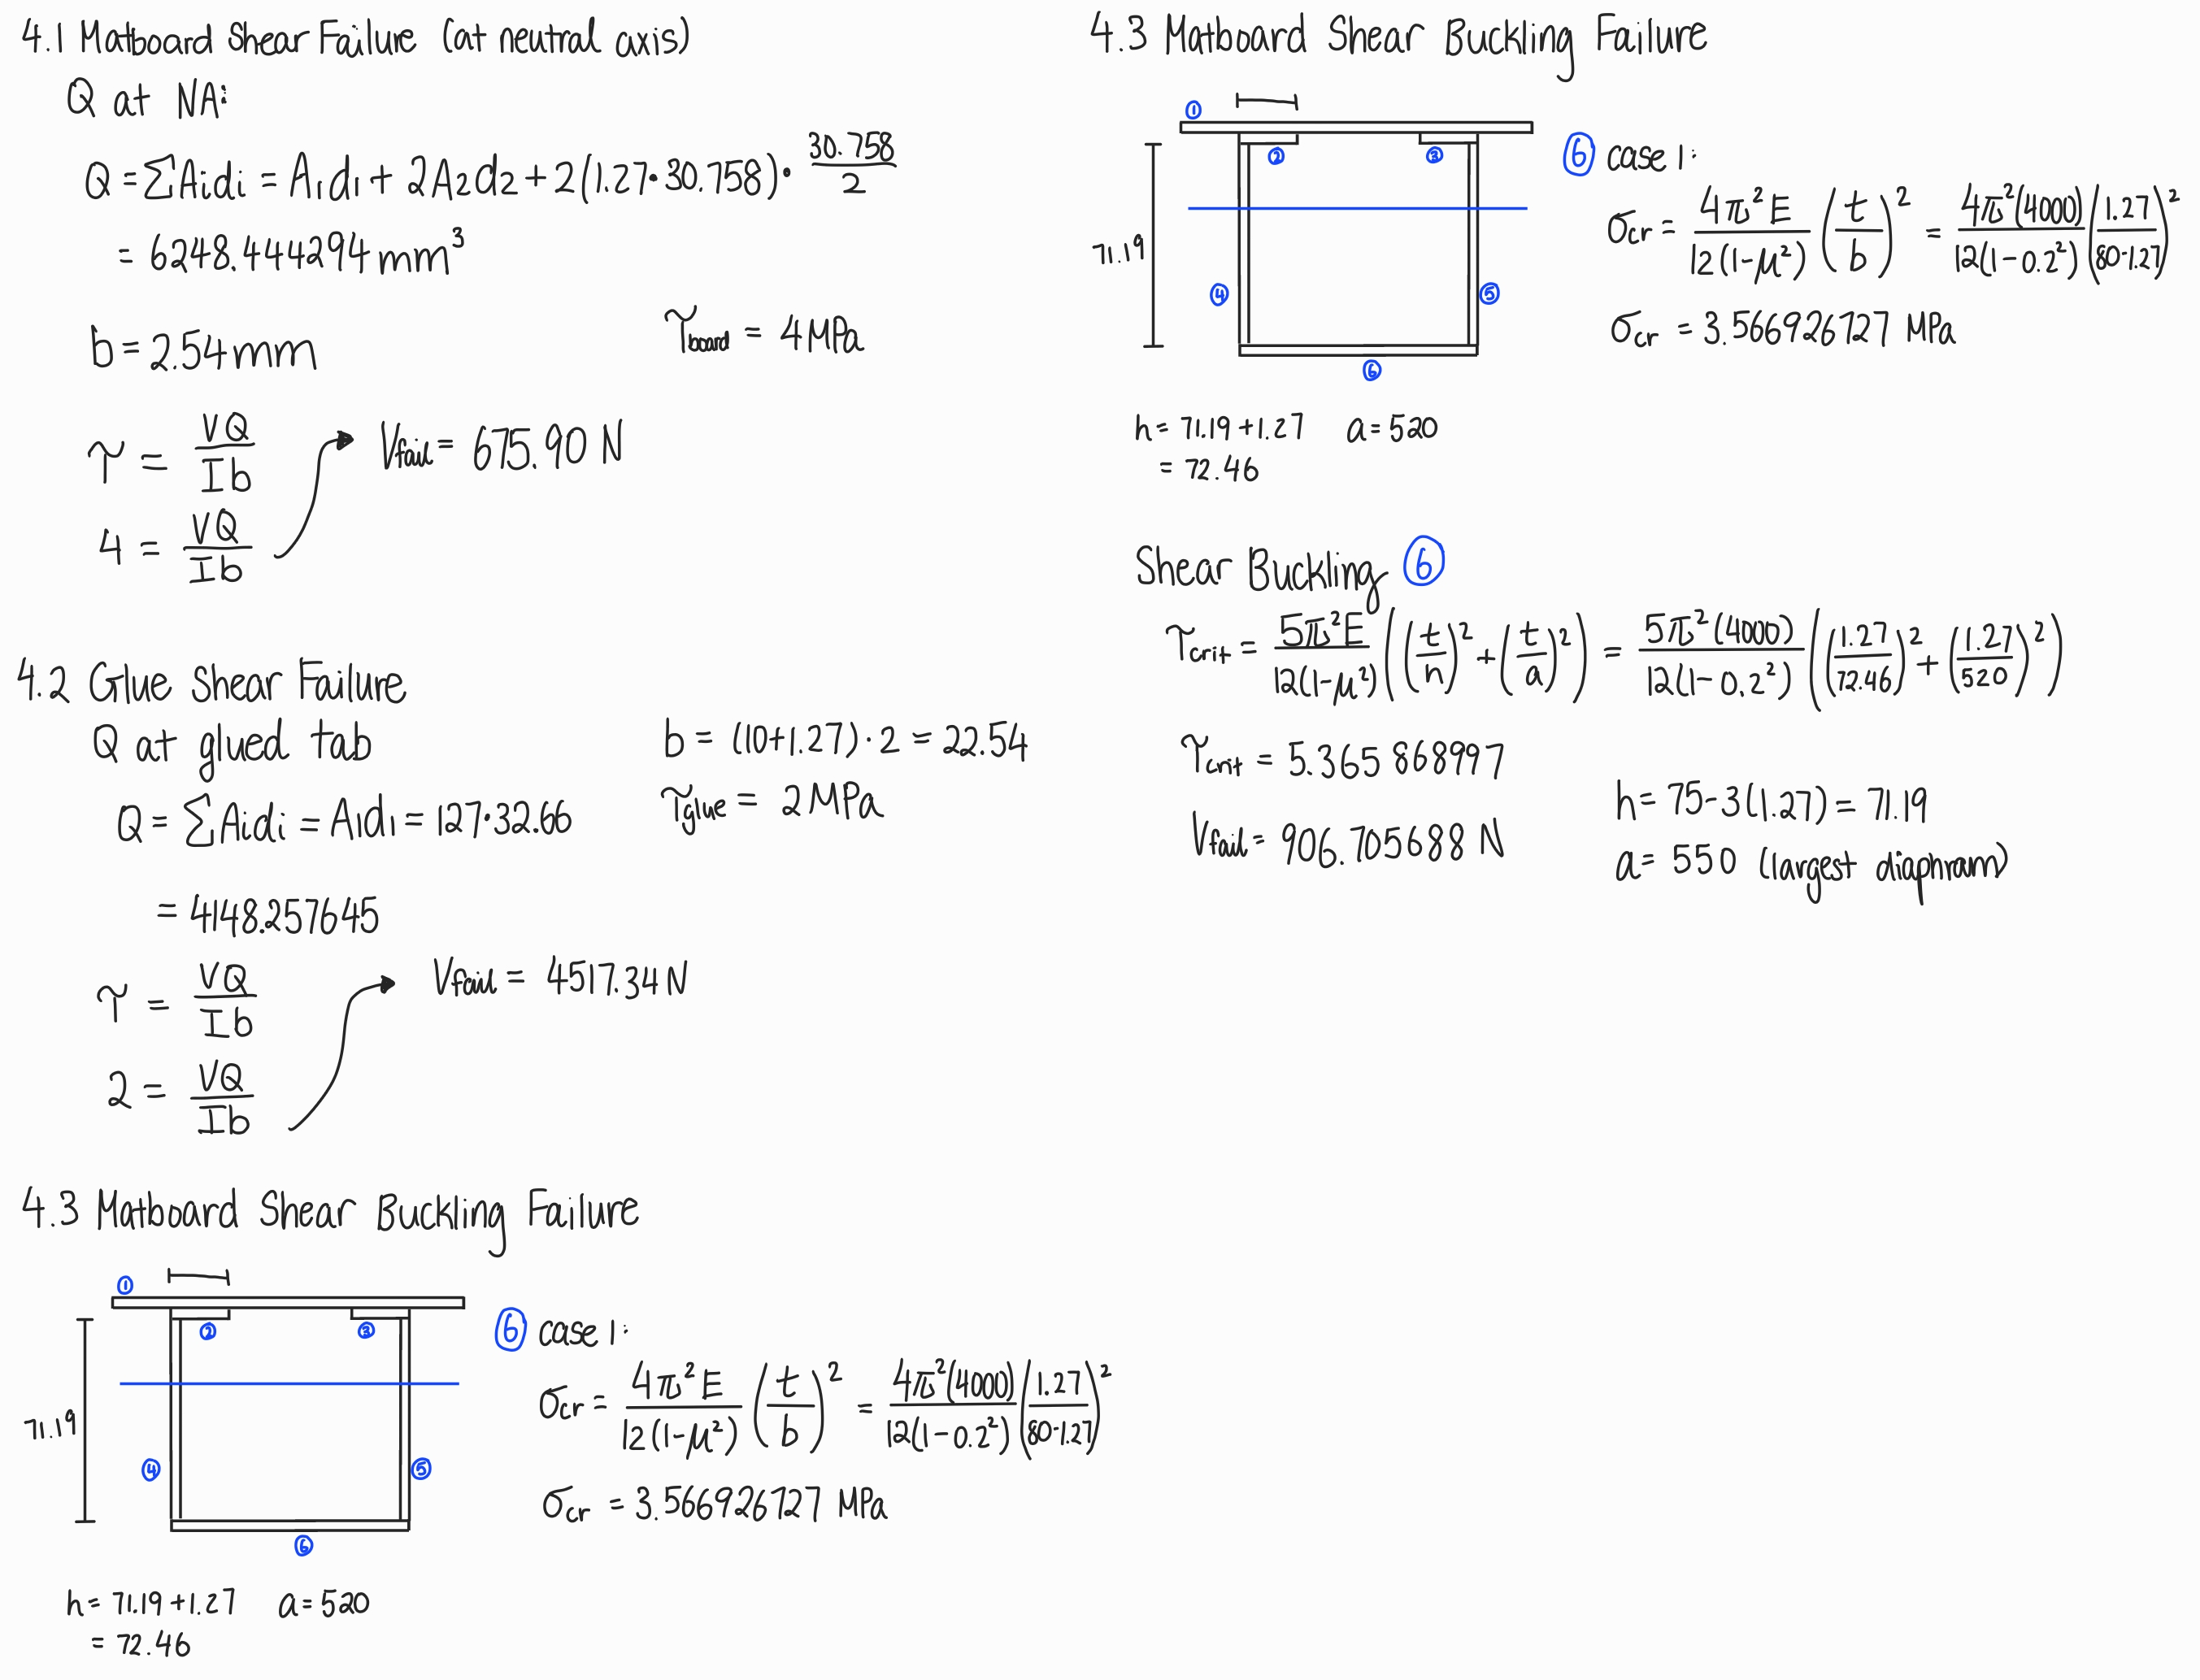
\includegraphics[width=\textwidth]{shear.png}
    \caption{Failure shear force calculations.}
\end{figure}

\subsubsection{Bending Moment Failure}

Note two values are calculated for each one because the values could be different depending on whether the top or the
bottom is in compression/tension.

\begin{alignat*}{2}
    \text{Tensile Failure: }&\sigma_t = \frac{M_{fail}y}{I} \implies M_{fail} = \frac{\sigma_t I}{y} &= \frac{30 \cdot 415685}{41.70} = \SI{229e3}{N.mm} \\
        & &= \frac{30 \cdot 415685}{41.70 - 75} = \SI{375e3}{N.mm} \\
    \text{Compressive Failure: }&\sigma_c = \frac{M_{fail}y}{I} \implies M_{fail} = \frac{\sigma_c I}{y} &= \frac{6 \cdot 415685}{41.70} = \SI{59.8e3}{N.mm} \\
        & &= \frac{6 \cdot 415685}{41.70 - 75} = \SI{74.9e3}{N.mm} \\
\end{alignat*}

\begin{figure}[H]
    \centering
    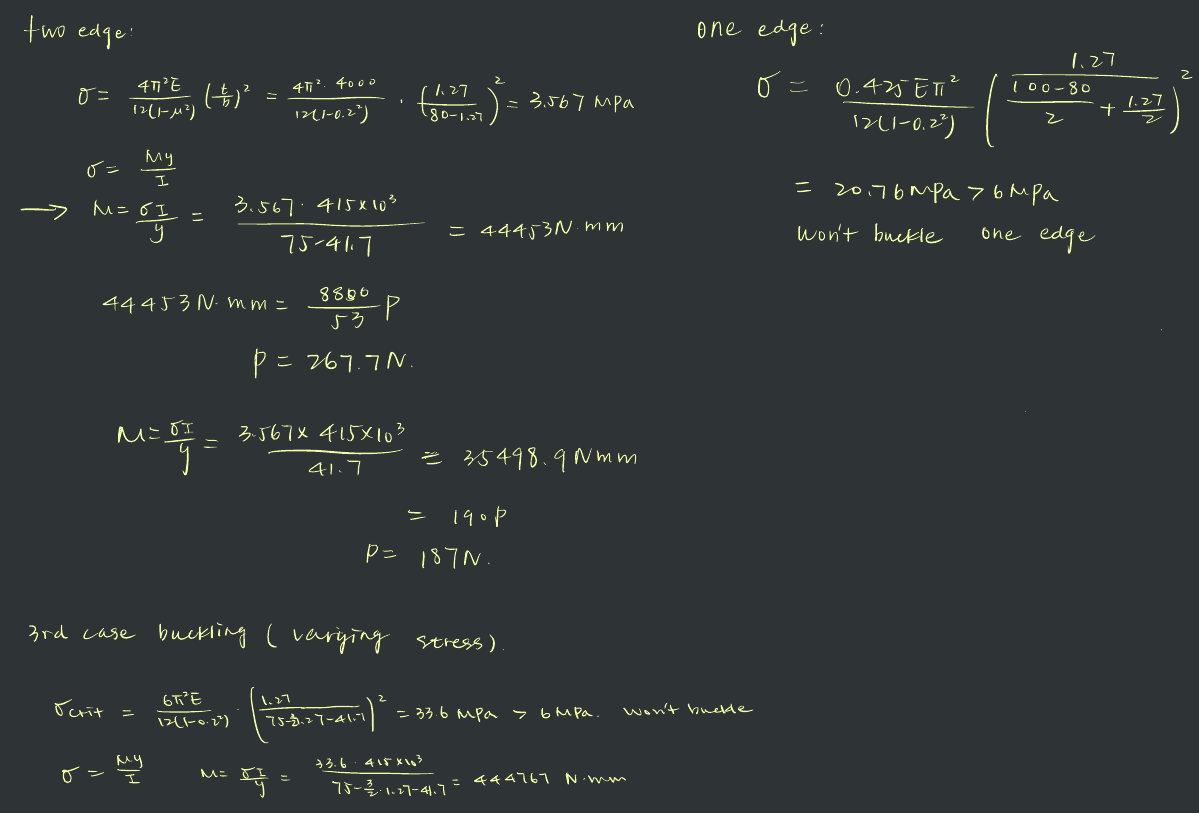
\includegraphics[width=\textwidth]{localbuckling.png}
    \caption{3 cases of local buckling.}
\end{figure}

\end{document}
